\section{Packet Capturing}
\label{packet_capture}
\subsection{Purpose}
In this experiment, we captured system's traffic data, then analyzed it to find the pattern of this IoT system communication. This packet data capturing method is also used in both “Device discovery experiment” and “Whitelist extraction experiment”. 

\begin{figure}[h]
    \centering 
    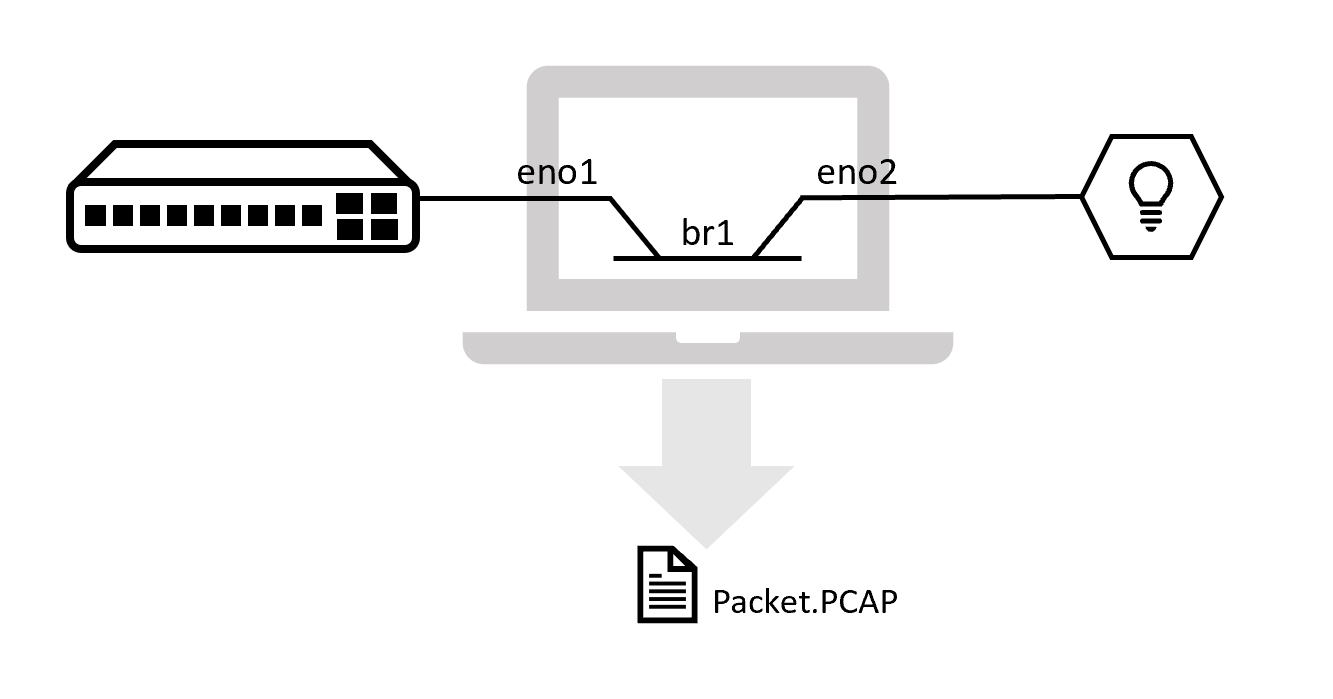
\includegraphics[width=0.65\textwidth]{4_packet_capturing}
    \caption{Packet Capturing}
    \label{fig:s4_packet_capturing}
\end{figure}


\subsection{Method}
First, we inserted a computer in between Switch and any IoT devices, we aim to capture its packet. As a requirement, computer used in this procedure must has at least 2 network interfaces. One network interface was connected to the switch, while another was connected to IoT device (Figure \ref{fig:s4_packet_capturing}). After that, we created network bridge to connect two of inserted computer network interfaces. Any computers run with Linux kernel can initiate a bridge using “brctl” command. Then packet would be captured using tpcdump command. (tcpdump is a TCP/IP packet sniffing command) Collected data was saved into PCAP format. 

In this experiment, we had tested capturing devices’ packet in 2 patterns. In pattern A (Figure \ref{fig:s4_pattern_a}), we created a computer bridge between all devices and switch, while in pattern B (Figure \ref{fig:s4_pattern_b}), we connected PC to one of IoT devices switch’s ports, and capturing packet coming through.

\begin{figure}[h]
    \centering
    \begin{subfigure}[b]{0.35\textwidth}
        \centering
        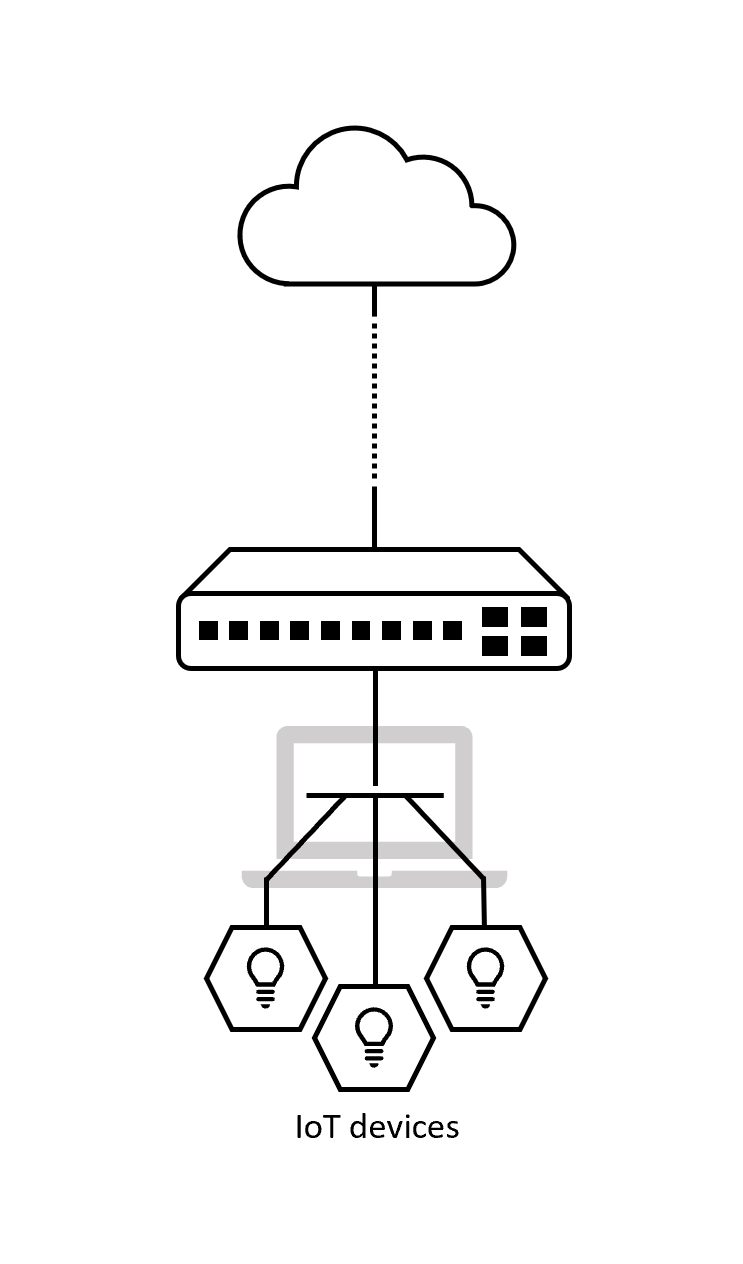
\includegraphics[width=\textwidth]{4_pattern_a}
        \caption{Pattern A: Capturing packets between switch and IoT devices}
        \label{fig:s4_pattern_a}
    \end{subfigure}
    \hspace{1.5cm}
    \begin{subfigure}[b]{0.35\textwidth}
        \centering
        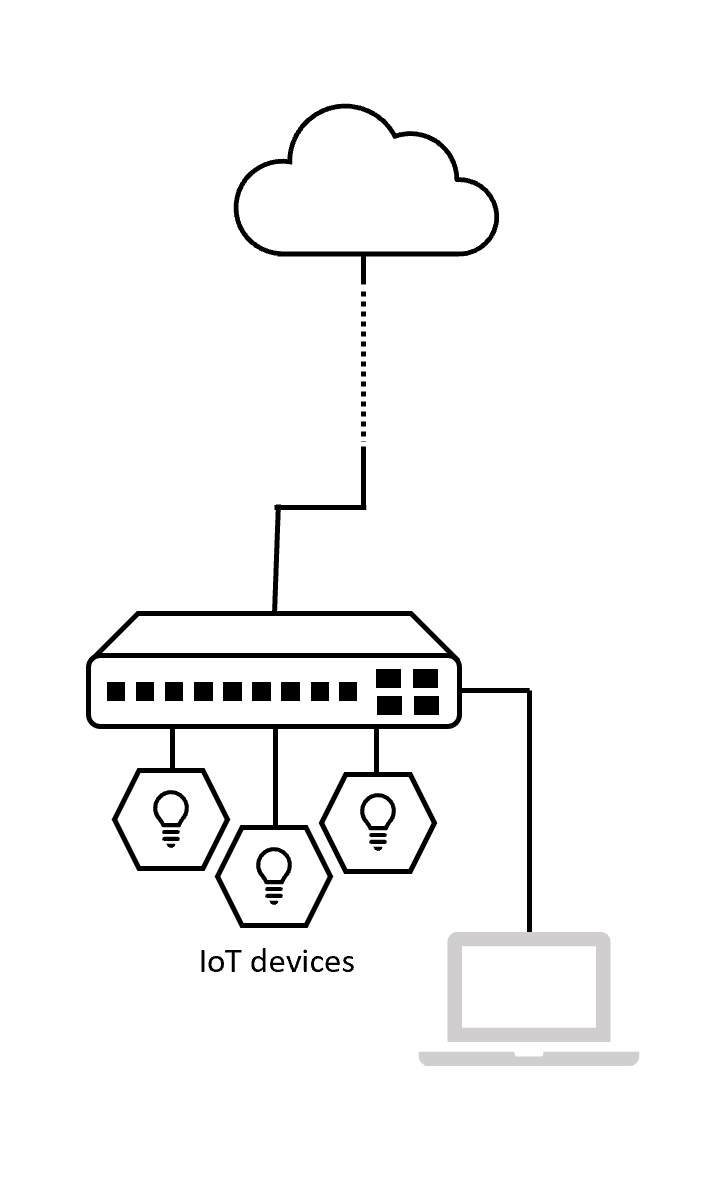
\includegraphics[width=\textwidth]{4_pattern_b}
        \caption{Pattern B: Capturing packet from one of switch's port}
        \label{fig:s4_pattern_b}
    \end{subfigure}
    \caption{Packet capturing method}
    \label{fig:s4_patterns}
\end{figure}



\subsection{Result}

After we have sufficiently taken to traffic data, we used Wireshark to perform primary investigation. 
The summary of each captured data is shown in table \ref{tab:s4_metadata}.

\begin{table}[H]
    \caption{Captured data summary}
    \begin{tabular*}{\textwidth}{l@{\extracolsep{\fill}}cc}
    \toprule
    & \textbf{Captured period} & \begin{tabular}[c]{@{}l@{}} \textbf{Number of packets} \end{tabular} \\ \toprule
    \textbf{Pattern A}  & 2018-11-29 07:21:26 - 2018-12-04 05:40:04 & 905454 \\ \hline
    \textbf{Pattern B}  & 2019-01-20 12:52:30 - 2019-01-20 17:49:45 & 6424 \\ \bottomrule
    \label{tab:s4_metadata}
\end{tabular*}

\end{table}

\subsubsection{Pattern A (Switch-Bridge-IoT)}
We analyzed network traffic data (Pattern A) and summarized each host necessary traffic in table \ref{tab:s4_eroom}.

\begin{table}[H]
    \caption{Pattern-A Packet Summary}
    \label{tab:s4_eroom}
    \begin{tabular}{l|lll}
    \toprule
    \textbf{Source}                                                                & \textbf{Destination}                                                                                             & \textbf{Protocol}   & \textbf{Description}                                                               \\ \toprule
    \multirow{3}{*}{Router(.1)}                                                     & 224.0.0.1                                                                                                        & IGMPv2              & \begin{tabular}[c]{@{}l@{}}Multi-cast group \\ participation protocol\end{tabular} \\ \cline{2-4} 
                                                                                   & 239.255.255.250                                                                                                  & SSDP(UDP/1900)     & \begin{tabular}[c]{@{}l@{}}Simple Service \\ Discovery Protocol\end{tabular}       \\ \cline{2-4} 
                                                                                   & EchonetLite \small(.10)                                                                                                & DNS(UDP/53)         & DNS Response                                                                       \\ \hline
    \multirow{4}{*}{\begin{tabular}[c]{@{}l@{}}EchonetLite\\ (.10)\end{tabular}}   & 160.16.109.189                                                                                                   & HTTP/POST(TCP/80)  & \begin{tabular}[c]{@{}l@{}}For saving data \\ to the database\end{tabular}         \\ \cline{2-4} 
                                                                                   & \begin{tabular}[c]{@{}l@{}}133.243.238.243,\\ 133.243.238.244,\\ 133.243.238.164,\\ 133.243.238.163\end{tabular} & NTP(UDP/123)        & Network Time Protocol                                                              \\ \cline{2-4} 
                                                                                    \small& Router \small(.1)                                                                                                       & DNS(UDP/53)         & DNS Query                                                                          \\ \cline{2-4} 
                                                                                   & \begin{tabular}[c]{@{}l@{}}\small Air Conditioner and \\ \small Control panel \\ \small (.12/.13 and .11)\end{tabular}                                             & Profinet(UDP/3610) & EchoNet Protocol                                                                   \\ \hline
    \multirow{2}{*}{\begin{tabular}[c]{@{}l@{}}Control panel\\ (.11)\end{tabular}} & 54.65.232.105                                                                                                   & HTTPs(TCP/443)     & TLSv1.2                                                                            \\ \cline{2-4} 
                                                                                   & 224.0.23.0                                                                                                       & IGMPv2              & \begin{tabular}[c]{@{}l@{}}Multi-cast group \\ participation protocol\end{tabular} \\ \cline{2-4}
                                                                                    & EchonetLite \small(.10)                                                                                                & Profinet(UDP/3610)         & DNS Response                                                                       \\ \hline
                                                                                \begin{tabular}[c]{@{}l@{}}Air Conditioner\\  (.12/.13)\end{tabular}           & EchonetLite \small(.10)                                                                                                & Profinet(UDP/3610) & EchoNet Protocol                                                           \\ \bottomrule       
    \end{tabular} 
    
\end{table}


\subsubsection{Pattern B (Switch Port)}
For pattern B, we could only detect broadcast packets. We found that packet data we have captured is mainly contained with ARP request packet and SSDP packet.
\newline\newline
From the result above, we knew which host is necessary for device and which is not.  
We would then use table \ref{tab:s4_eroom} as the evaluator for our "Whitelist Extraction" experiment (section \ref{s4:whitelist})  
